\chapter{Supercontinuum Generation}
\label{ch:supercontinuum}

Previous chapters explained individual linear and nonlinear effects and the interplay of a limited number of them. A summary of their impacts is provided in Tab.~\ref{tab:NL_summary}. For high power pulses with carrier frequencies where $\betag_2\lesssim 0$ and $\gamma>0$ for a given medium as well as durations below approximately 100~fs, all of the listed effects may be present simultaneously. In this case, the evolution of the pulse may be highly non-trivial and broaden its spectrum by ten to twenty times its initial bandwidth~\cite{supercontinuum_original_paper}. This chapter presents an example of supercontinuum generation and explains how this process can be understood in terms of the previously presented effects.   

\begin{table}[]
\begin{adjustwidth}{-2cm}{}
\begin{tabular}{ccccc}
\hline
\textbf{Effect}       & \textbf{Time domain}                                                                                      & \textbf{Spectrum}                                                                                           & \textbf{Significant for}                                                                           & \textbf{Relevance}                                                                                                       \\ \hline
$\alpha>0$            & Increase power.                                                                                           & Increase power.                                                                                             & Amplifiers                                                                                         & \begin{tabular}[c]{@{}c@{}}NL effects highly \\ power dependent.\end{tabular}                                            \\ \hline
$\beta_2<0$           & \begin{tabular}[c]{@{}c@{}}Broadening with \\ blue(red)  light in \\ front(back).\end{tabular}            & \begin{tabular}[c]{@{}c@{}}Quadratic change \\ in phase with \\ distance from \\ carrier freq.\end{tabular} & \begin{tabular}[c]{@{}c@{}}Short NIR pulses \\ in silica.\end{tabular}                             & \begin{tabular}[c]{@{}c@{}}NL effects significant \\ when $\beta_2+\gamma P\approx 0$.\end{tabular}                      \\ \hline
$\beta_3$             & \begin{tabular}[c]{@{}c@{}}Delays or advances \\ non-carrier freqs. \\ depending on sign.\end{tabular}    & \begin{tabular}[c]{@{}c@{}}Cubic change in \\ phase with distance \\ from carrier freq.\end{tabular}        & \begin{tabular}[c]{@{}c@{}}Carrier freqs. \\ close to ZDF.\end{tabular}                            & \begin{tabular}[c]{@{}c@{}}Different freqs. \\ overlapping in time \\ domain cause FWM. \\ Soliton fission.\end{tabular} \\ \hline
Self Phase Modulation & \begin{tabular}[c]{@{}c@{}}Red(blue)-shift on \\ leading(trailing)edges.\end{tabular}                     & \begin{tabular}[c]{@{}c@{}}Symmetric \\ broadening.\end{tabular}                                            & High power pulses                                                                                  & \begin{tabular}[c]{@{}c@{}}Most basic NL effect. \\ First to "kick in" as \\ power is increased.\end{tabular}            \\ \hline
Self Steepening       & \begin{tabular}[c]{@{}c@{}}Pulse peak delayed \\ to later times causing \\ steep back slope.\end{tabular} & \begin{tabular}[c]{@{}c@{}}Broadening skewed \\ towards higher \\ frequencies.\end{tabular}                 & \begin{tabular}[c]{@{}c@{}}Pulses with short \\ duration compared \\ to carrier freq.\end{tabular} & \begin{tabular}[c]{@{}c@{}}Small correction on \\ top of SPM.\\ Soliton fission.\end{tabular}                            \\ \hline
Raman                 & Red-shift at pulse peak.                                                                                  & \begin{tabular}[c]{@{}c@{}}Broadening skewed \\ towards lower \\ frequencies.\end{tabular}                  & \begin{tabular}[c]{@{}c@{}}Extremely short \\ pulses on the scale \\ of 10-100fs.\end{tabular}     & \begin{tabular}[c]{@{}c@{}}Raman red-shift can \\ exceed SPM \\ broadening.  \\ Soliton fission.\end{tabular}            \\ \hline
\end{tabular}
\caption{Summary of the impacts of different linear and nonlinear effects.}
\label{tab:NL_summary}
\end{adjustwidth}
\end{table}
\section{Case study}
To simulate the generation of a supercontinuum, the values in Tab.~\ref{tab:SC_params} were used. The resulting supercontinuum is presented in Fig.~\ref{fig:SC_combined}. The spectrum in Fig.~\ref{fig:SC_combined} c) indicates that the pulse undergoes SPM during the first 1~m of propagation, while Fig.~\ref{fig:SC_combined} b) indicates that soliton fission occurs immediately afterwards. The high-power pulse with a much smaller duration that walks off parabolically towards later times is a Raman soliton that continuously red-shifts itself. The low-power light that "walks off" linearly towards later times is most likely FWM generated when the fissioned soliton overlaps with the remnants of the initial pulse. See \href{https://youtu.be/-GDsMDpC3oA}{this video tutorial} for an in-depth analysis of the properties of this supercontinuum.

\begin{table}[]
\centering
\begin{tabular}{cc}
\textbf{Parameter}                      & \textbf{Value}                                  \\ \hline
N time points                           & $2^{14}$                                          \\
Time resolution {[}fs{]}                & 1.8                                             \\\hline
Pulse type                              & Sech                                            \\
Duration {[}fs{]}                       & 166.79                                          \\
Peak Power {[}W{]}                      & 50                                              \\
Carrier freq. {[}THz{]}                 & 282.823 (=1060~nm)                         \\\hline
$\alpha$ {[}dB/km{]}                    & 0                                               \\
$\betag_2$ {[}s\textasciicircum{}2/m{]} & -3.051721e-27                                   \\
$\betag_3$ {[}s\textasciicircum{}3/m{]} & 7.29029e-41                                     \\
$\betag_4$ {[}s\textasciicircum{}4/m{]} & -1.08817e-55                                    \\
$\betag_5$ {[}s\textasciicircum{}5/m{]} & 2.8941e-70                                      \\
$\betag_6$ {[}s\textasciicircum{}6/m{]} & 4.8348e-89                                      \\
$\betag_7$ {[}s\textasciicircum{}7/m{]} & -1.1464e-113                                    \\
$\betag_8$ {[}s\textasciicircum{}8/m{]} & 1.8802e-128                                     \\
$\betag_9$ {[}s\textasciicircum{}9/m{]} & -1.5054e-143                                    \\
$\gamma$ {[}1/W/m{]}                    & 0.09                                            \\
Self-Steepening                         & ON                                              \\
Raman model                             & Eq.~\ref{eq:raman_basic}
\end{tabular}
\caption{Simulation parameters used for generating a supercontinuum taken from~\cite{supercontinuum_paper}}
\label{tab:SC_params}
\end{table}

\begin{figure}
    \centering
    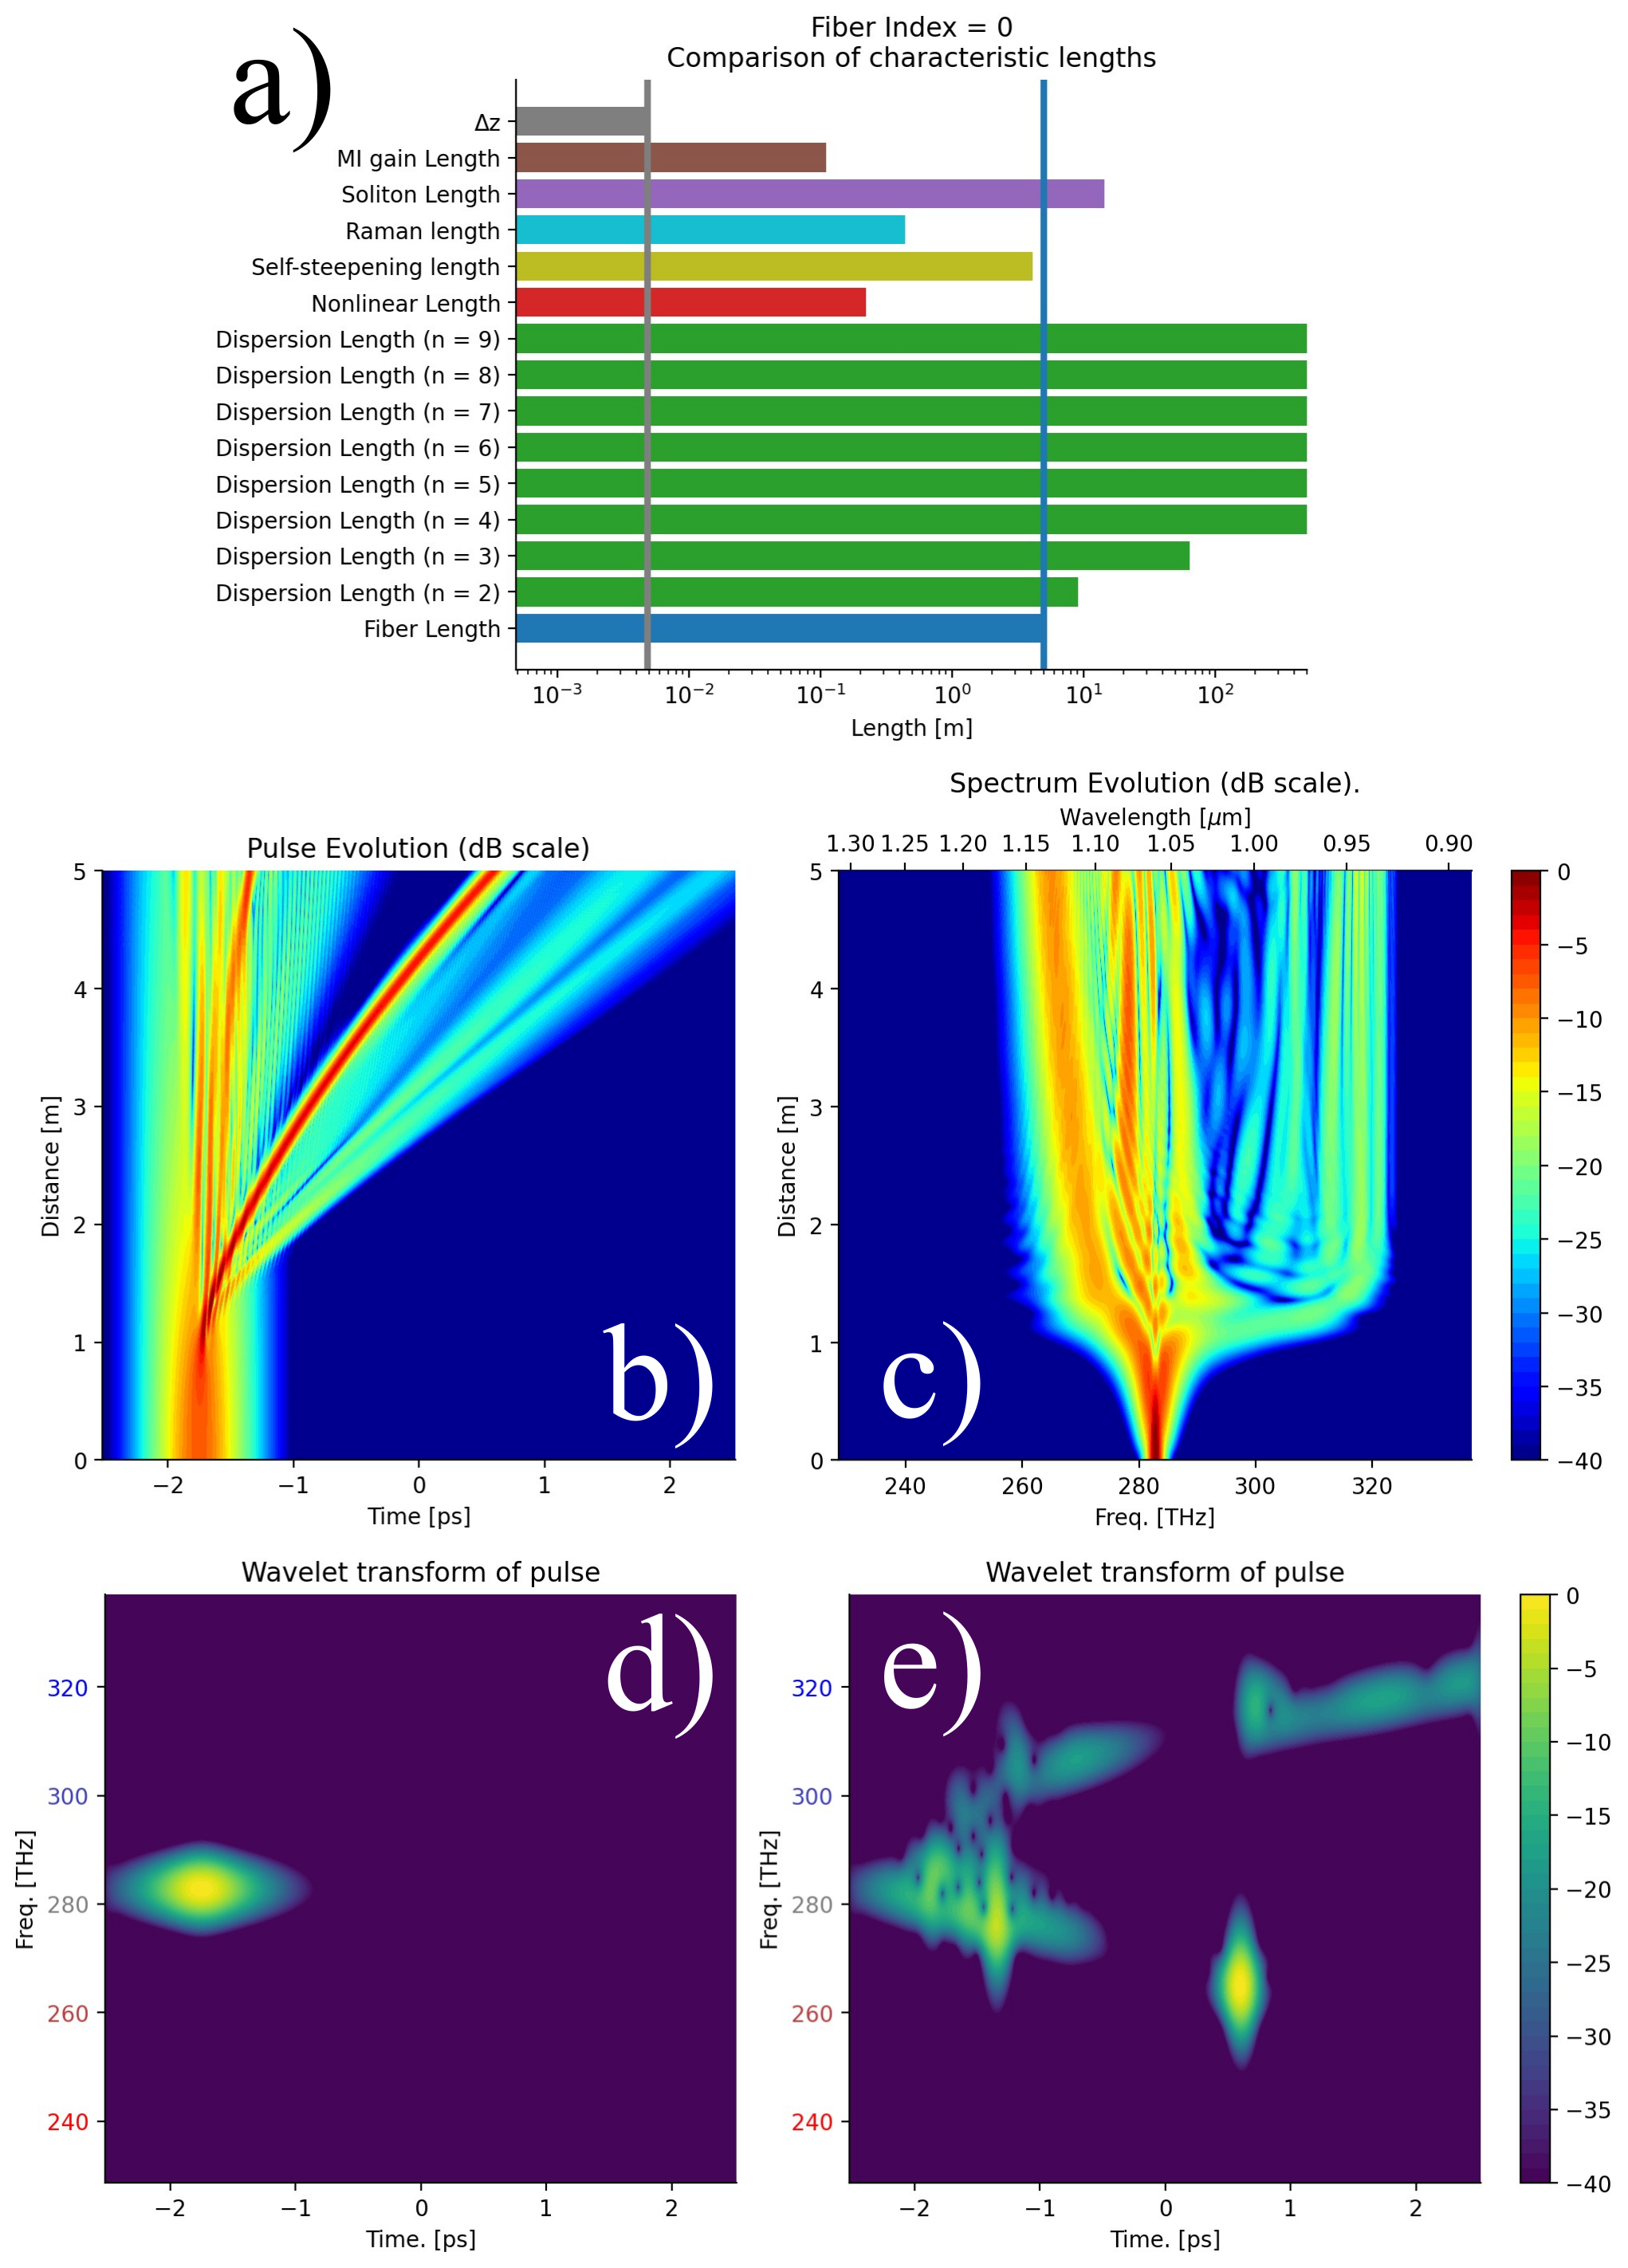
\includegraphics[width=0.9\linewidth]{figures/SC_combined.png}
    \caption{a) Comparison of the characteristic lengths resulting from the parameters listed in Tab.~\ref{tab:SC_params}. Effects with short characteristic lengths are expected to become significant first. b) Temporal evolution of the pulse showing soliton fission at a distance of around 1~m followed by FWM and the generation of a Raman soliton walking off to later times. c) Spectral evolution of the pulse. d) Initial spectrogram of the pulse at z=0m. e) Final spectrogram at z=5m. The "parabolic" shape arises because $\betag_3>0$ ensures that both red and blue light experience time delays compared to the carrier. The bright spot at (0.75~ps, 265~THz) is a Raman soliton. Figures generated using the numerical simulation presented in \href{https://colab.research.google.com/drive/1HvA8F8yzEq-9fahuI4z2KhT-YhdRAXgt?usp=sharing}{this interactive notebook}, which the reader is encouraged to experiment with. }
    \label{fig:SC_combined}
\end{figure}

\section{Your turn!}
To further explore the properties of the supercontinuum modelled in Fig.~\ref{fig:SC_combined}, open the \href{https://colab.research.google.com/drive/1HvA8F8yzEq-9fahuI4z2KhT-YhdRAXgt?usp=sharing}{notebook} used for generating it, try the following experiments and explain how/why the evolution of the pulse and its spectrum are different. Before starting any experiment, write down a prediction of how you expect the simulation result to be altered, so you can compare with the actual result. Note that you should "reset" the parameters to the default values before each experiment:

\begin{enumerate}

\item \textbf{No nonlinearity}. The presented simulation uses $\gamma>0$. Change this to $\gamma=0$. Does the result indicate that nonlinearity has a large impact on the time evolution of the pulse?

\item \textbf{No Self-Steepening}. The presented simulation models the impact of self-steepening. Turn this effect off and asses if doing so had a significant impact.

\item \textbf{Negative $\alpha$}. The presented simulation uses $\alpha=0$. Change this to $\alpha=-1$~dB/m. 



\item \textbf{Positive $\betag_2$}. The presented simulation uses $\betag_2<0$. Change the sign of $\betag_2$ so it becomes positive. 



\item \textbf{Only $\betag_2<0$}. The presented simulation uses $\betag_n\neq0$ for $n>2$. Set $\betag_n = 0$ for $n>2$, run the simulation and explain why the evolution of the pulse and its spectrum has changed. 

\item \textbf{Negative $\betag_3$}. The presented simulation uses $\betag_3>0$. Change the sign of $\betag_3$ so it becomes positive. Note that you may want to change the sign of the time offset from -1.75~ps to +1.75~ps to ensure proper graphing of the time evolution. Can you explain why a Raman soliton does not arise when $\betag_3<0$? HINT: Compute the zero dispersion frequency using Eq.~\ref{eq:ZDF} and consider how it changes when the sign of $\betag_3$ is flipped.


\item \textbf{Alter the Raman model}. The presented simulation uses Eq.~\ref{eq:raman_basic} to model the impact of the Raman effect. Follow the hints in the notebook and use Eq.~\ref{eq:raman_new}, Eq.~\ref{eq:Raman_exact} or $f_R=0$ instead.  
\end{enumerate}